\epigraph{\textit{We cannot solve problems with the kind of thinking we employed when we came up with them.}}{-- \textup{Albert Einstein}}

In the following paragraphs, we are covering the motivation, contributions and structure of this document. This means, after reading it, you are building the big picture; a general idea of the motivations to develop this project, the goal we are looking forward to achieving and the shape of the document itself.

\section{Motivation}

A famous mathematical problem from the past is \textbf{The Seven Bridges of Königsberg}. The foundations of \textit{graph theory} were set by Leonhard Euler's negative resolution\footnote{The \textbf{negative resolution} system consists of applying the resolution rule where one of the clauses being a negative literal.} to the problem in 1736.

The city of Königsberg in Prussia (now Kaliningrad, Russia) was built on both banks of the \textit{Pregel River} and featured two sizable islands, Kneiphof and Lomse, which were linked to the two mainland sections of the city by seven bridges. The challenge was creating a route through the city that would cross each of those bridges just once. What Euler proved was that this problem has no solution.

\begin{figure}[ht]
    \begin{subfigure}{.3\textwidth}
        \centering
        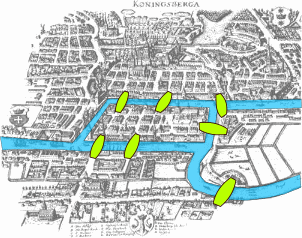
\includegraphics[width=.7\linewidth]{img/4-1_konigsberg_bridges.png}
        \caption{The seven bridges' exact positioning is shown on Königsberg's map from Euler's time, highlighting the Pregel River in blue}
    \end{subfigure}%
    \hspace*{0.5em}
    \begin{subfigure}{.3\textwidth}
        \centering
        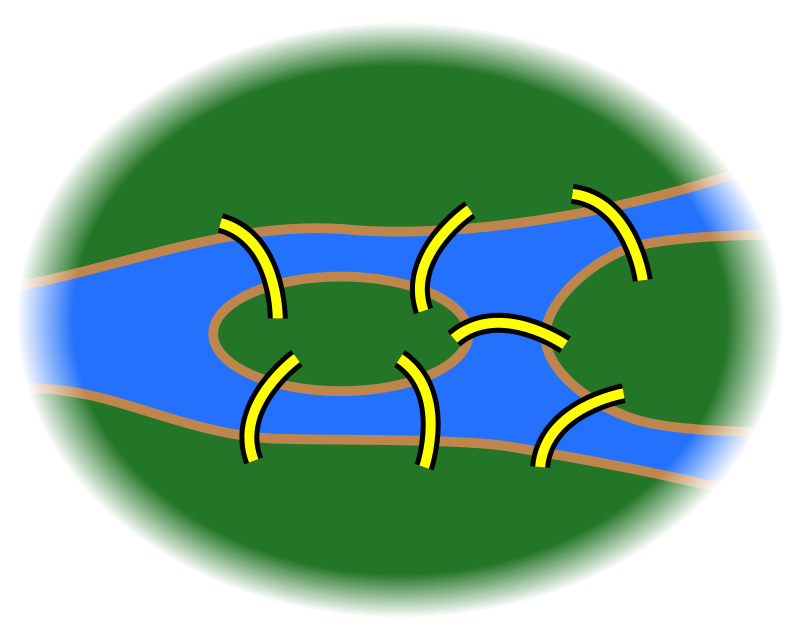
\includegraphics[width=.7\linewidth]{img/4-2_konigsberg_abstract.png}
        \caption{Diagram illustrating The Seven Bridges of Königsberg's puzzle. Take note of how our level of abstraction has increased}
    \end{subfigure}%
    \hspace*{0.5em}
    \begin{subfigure}{.3\textwidth}
        \centering
        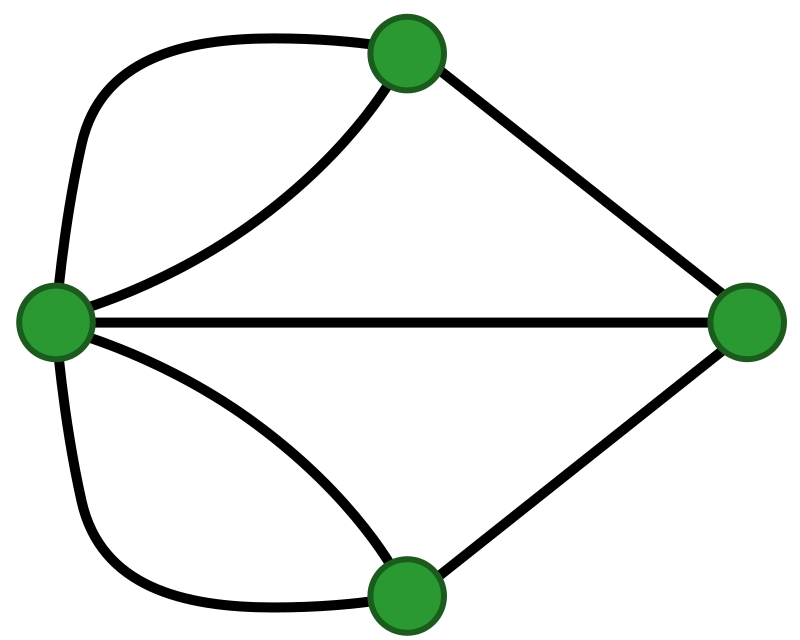
\includegraphics[width=.7\linewidth]{img/4-3_konigsberg_graph.png}
        \caption{Abstract graph corresponding to the bridges of Königsberg, where edges are de bridges and nodes are the sectors of the city}
    \end{subfigure}%
    \caption[Creating the equivalent graph of the problem of The Seven Bridges of Königsberg]{Creating the equivalent graph of the problem of The Seven Bridges of Königsberg\footnotemark}
\end{figure}
\footnotetext{\url{https://en.wikipedia.org/wiki/Seven_Bridges_of_Konigsberg}}

\subsection{Eueler's analysis}

In modern terms, Euler observed that the degree of the nodes; that is, the number of vertices connected to a particular element, determines the possibility of a walk around a graph, traversing each edge precisely once. According to Euler's theory, a connected graph with exactly zero or two nodes with odd degrees is a requirement for the walk around the entire network. This is because we can only cross each bridge once, therefore each traversal of a section of the city requires an even number of edges to be crossed. For each entrance on a mainland, we must enter through one bridge and exit through another. It turns out that this condition is also sufficient. We also know that if there are nodes with odd degrees, then any path will begin at one of them and end at the other. A path like this is currently known as the Eulerian path and is named after the mathematician. Summing up, we have proved that there can be no Eulerian path in the graph that corresponds to Königsberg since it contains four nodes of odd degrees.

\section{Project Scope}

A growing number of devices are interconnected, these days. As a result, tons of data is being automatically stored. This way, processing that data becomes both a more challenging and important task. Simply stated, the amount of data we try to handle outruns our capacity to consume it. Big data, a new area of software development, where we quickly handle large volumes of heterogeneous information, offers a remedy for this.

Interoperability is a crucial subject we must deal with in big data applications since they not only need to scan huge volumes of inputs as quickly as possible but also because the information comes from a range of sources.

Knowledge graphs~\cite{https://doi.org/10.48550/arxiv.2110.11709} were popularized back in 2012 by Google~\cite{web:knowledge_graphs:google} as a tool to represent real-world data reflecting relationships between entities to understand those links better. After Google's introduction, others embraced this approach: ranging from proprietary to open databases. Being the content of the latter publicly available. Prominent companies -- including \textit{web search} (e.g., Bing~\cite{knowledge:graphs:usage:bing} and Google~\cite{web:knowledge_graphs:google}), \textit{commerce} (e.g., Airbnb~\cite{knowledge:graphs:usage:airbnb} and Amazon~\cite{knowledge:graphs:usage:amazon}), \textit{social networks} (e.g., Facebook~\cite{knowledge:graphs:usage:facebook} and LinkedIn~\cite{knowledge:graphs:usage:linkedin}) or \textit{finances} (e.g., Accenture~\cite{knowledge:graphs:usage:accenture} and Banca d'Italia~\cite{https://doi.org/10.48550/arxiv.2010.05172}) -- are using knowledge graphs to have a better understanding of their customers. Even though there exist several models associated with this technology, we are focusing on Wikibase graphs.

Summing up, this project focuses on the analysis and implementation of a system to validate Wikibase graphs -- a specific flavor of the so-called knowledge graphs -- using big data techniques. To put that into perspective, as of October 1, 2022, a compressed dump\footnote{A \textbf{dump} is a copy of the whole Wikibase raw data that can be downloaded from their system. This could also be understood as a snapshot of what was stored in the system at a certain moment} of Wikidata's database has a size of 109.04GB~\cite{wikidata:dumps}. Not only that, but the size of these dumps has exponentially increased with every release (see Figure \ref{fig:dumps}).

\begin{figure}[ht]
    \centering
    \includestandalone[width=0.4\textwidth]{diagrams/1-1_dumps}
    \caption[Plot showing the size of compressed dumps between 2014-22]{Size of compressed Wikidata dumps between 2014-2022~\cite{https://doi.org/10.48550/arxiv.2110.11709}}
    \label{fig:dumps}
\end{figure}

These enormous sizes make it difficult for users to easily examine and process the content of them, and they also raise the possibility that these technologies will become victims of their success. This condition is demonstrated in Scholia, an online application that uses Wikidata to describe data about academics and their works. The app includes appealing visualizations and comparisons that are based on requests through the Wikidata endpoint. Despite the project offering a wealth of intriguing data, timeouts caused by the massive volumes of information prevent access to the most intricate visualizations.

Creating subsets of the Knowledge Graphs for specific domains may be one solution to these problems. These subsets serve as snapshots of the data at certain points in time and can be used to enhance the performance of the apps that consume that data, making it easier to research the contents of Knowledge Graphs.

\label{section:objectives}
\section{Objectives}

\paragraph{Project's Goal 1}
\textit{Design and implementation of a system for validating huge dumps from Wikidata generating a subset out of it.} As we have stated during these introductory lines, the task of having to process enormous amounts of data is becoming increasingly relevant. The faster a system allows us to accomplish it, the better solution we will provide. We are not only interested in Wikidata dumps but also other Knowledge graphs. The more generic the solution is, the better.

\paragraph{Project's Goal 2}
\textit{Reproduce an experiment related to the analysis of the previously described algorithm.} For us to properly analyze the results emerging from the execution of the algorithm we have implemented, we have to create an ecosystem where we can obtain information related to memory consumption or execution time, to name a few. This way, we are willing to create a solution that is capable of being executed in commodity hardware.

\paragraph{Project's Goal 3}
\textit{Learn new technologies and Big data techniques.} As this is an academic project and one of the main objectives of a research project is finding innovative solutions to a certain problem: learning and exploring new possibilities is -- indeed -- one of this project's goals.

\section{Contributions}

Having the main objective and motivations introduced, let me highlight the key contributions of this project. Take note that the document is divided into several parts, one per each of the contributions listed below.

\begin{enumerate}
    \itemsep0.5em
    \item Research and documentation of the existing method for validating Wikibase Knowledge Graphs provided a schema that the graph's entities should conform to. The suggested solution is implemented in Scala and Apache Spark; yet, at the project's first meeting, several proposals for enhancing the real solution were presented. The original code was rewritten according to the aforementioned research, although the resulting solution was far from ideal. The process of exploring and refactoring the code is enumerated in the chapters to come.
    \item Presentation of a novel Rust and SQL-based Knowledge Graph subset generation architecture. The goal is to provide a solution that can run on any hardware efficiently. We are willing to explore the capabilities of Rust for enabling some performance gains regarding single-node computation. What's more, when comparing them to NoSQL, relational databases are on the rise. According to some early findings, the JSON dump is 10 times larger in size than the generated single database file. More on this will be discussed in the following chapters.
\end{enumerate}

\section{Structure of the document}

The shape of this document is as follows:

\begin{itemize}
    \itemsep0.25em
    \item[\textbf{Chapter ~\ref{chapter:related}.}] General description of the existing technologies related to knowledge graph validation. As well as the advantages and disadvantages of choosing some tools over others for implementing this project.
    \item[\textbf{Chapter ~\ref{chapter:theory}.}] Provides a theoretical background needed for a better understanding of the concepts explained in the following chapters.
    \item[\textbf{Chapter ~\ref{chapter:existing}.}] Description of the initial solution implemented by Labra, serving as the project's baseline.
    \item[\textbf{Chapter ~\ref{chapter:refactoring}.}] Description of the changes introduced to the original solution, as well as the reasons behind them.
    \item[\textbf{Chapter ~\ref{chapter:analysis}.}] Analysis of the new perspective introduced by the final solution. As well as the advantages and disadvantages of choosing some tools over others for implementing this project.
    \item[\textbf{Chapter ~\ref{chapter:wd2duckdb}.}] Description of the process followed to create the new solution based on Rust and DuckDB.
    \item[\textbf{Chapter ~\ref{chapter:pschema}.}] Explanation of the process followed to create the algorithm that validates the knowledge graphs.
    \item[\textbf{Chapter ~\ref{chapter:experiment}.}] Explanation of the process followed to analyze the concrete implementation of the algorithm that we used to validate the knowledge graphs.
    \item[\textbf{Chapter ~\ref{chapter:results}.}] Analysis of the results obtained from the previously described experiment.
    \item[\textbf{Chapter ~\ref{chapter:planning}.}] Summary of the process followed to create this final degree project, as well as some considerations regarding management and organization of resources.
    \item[\textbf{Chapter ~\ref{chapter:conclusions}.}] Summary of the general conclusions and future work.
\end{itemize}